%%%% Paramétrage du cours %%%%
\def\xxactivite{Cours}
\def\xxauteur{\textsl{Xavier Pessoles}}

\fichefalse \proftrue \tdfalse \courstrue

\def\xxnumchapitre{Chapitre 2 \vspace{.2cm}}
\def\xxchapitre{\hspace{.12cm} Correction numérique des systèmes asservis}

\def\xxcompetences{%
\textsl{%
\textbf{Savoirs et compétences :}\\
\begin{itemize}[label=\ding{112},font=\color{ocre}] 
\item B2-09 : Modéliser un correcteur numérique :
\begin{itemize}
\item caractérisation des signaux à temps discret (échantillonnage et quantification);
\item modélisation par équations aux différences (équations de récurrence) d'un correcteur numérique (proportionnel, proportionnel intégral et à avance de phase).
\end{itemize}
\end{itemize}
}}


\def\xxfigures{
%\includegraphics[width=3cm]{SoloWheel_Orbit}%
%\\
%\textit{SoloWheel Orbit.}
}%figues de la page de garde


\pagestyle{empty}


%%%%%%%% PAGE DE GARDE COURS
\ifcours
\begin{tikzpicture}[remember picture,overlay]
\node at (current page.north west)
{\begin{tikzpicture}[remember picture,overlay]
\node[anchor=north west,inner sep=0pt] at (0,0) {\includegraphics[width=\paperwidth]{\thechapterimage}};
\draw[anchor=west] (-2cm,-8cm) node [line width=2pt,rounded corners=15pt,draw=ocre,fill=white,fill opacity=0.6,inner sep=40pt]{\strut\makebox[22cm]{}};
\draw[anchor=west] (1cm,-8cm) node {\huge\sffamily\bfseries\color{black} %
\begin{minipage}{1cm}
\rotatebox{90}{\LARGE\sffamily\textsc{\color{ocre}\textbf{\xxnumpartie}}}
\end{minipage} \hfill
\begin{minipage}[c]{14cm}
\begin{titrepartie}
\begin{flushright}
\renewcommand{\baselinestretch}{1.1} 
\Large\sffamily\textsc{\textbf{\xxpartie}}
\renewcommand{\baselinestretch}{1} 
\end{flushright}
\end{titrepartie}
\end{minipage} \hfill
\begin{minipage}[c]{3.5cm}
{\large\sffamily\textsc{\textbf{\color{ocre} \discipline}}}
\end{minipage} 
 };
\end{tikzpicture}};
\end{tikzpicture}


\begin{tikzpicture}[overlay]
\node[shape=rectangle, 
      rounded corners = .25 cm,
	  draw= ocre,
	  line width=2pt, 
	  fill = ocre!10,
	  minimum width  = 2.5cm,
	  minimum height = 3cm,] at (18cm,0) {};
\node at (17.7cm,0) {\rotatebox{90}{\textbf{\Large\color{ocre}{\classe}}}};
%{};
\end{tikzpicture}

\vspace{3.5cm}

\begin{tikzpicture}[remember picture,overlay]
\draw[anchor=west] (-2cm,-6cm) node {\huge\sffamily\bfseries\color{black} %
\begin{minipage}{2cm}
\begin{center}
\LARGE\sffamily\textsc{\color{ocre}\textbf{\xxactivite}}
\end{center}
\end{minipage} \hfill
\begin{minipage}[c]{15cm}
\begin{titrechapitre}
\renewcommand{\baselinestretch}{1.1} 
\Large\sffamily\textsc{\textbf{\xxnumchapitre}}

\Large\sffamily\textsc{\textbf{\xxchapitre}}
\vspace{.5cm}

\renewcommand{\baselinestretch}{1} 
\normalsize\normalfont
\xxcompetences
\end{titrechapitre}
\end{minipage}  };
\end{tikzpicture}
\vfill

\begin{flushright}
\begin{minipage}[c]{.3\linewidth}
\begin{center}
\xxfigures
\end{center}
\end{minipage}\hfill
\begin{minipage}[c]{.6\linewidth}
\startcontents
\printcontents{}{1}{}
\end{minipage}
\end{flushright}

\begin{tikzpicture}[remember picture,overlay]
\draw[anchor=west] (4.5cm,-.7cm) node {
\begin{minipage}[c]{.2\linewidth}
\begin{flushright}

\includegraphics[width=2cm]{png/logoCC}
\end{flushright}
\end{minipage}
\begin{minipage}[c]{.2\linewidth}
\textsl{\xxauteur} \\
\textsl{\classe}
\end{minipage}
 };
\end{tikzpicture}
\newpage
\pagestyle{fancy}

\newpage
\pagestyle{fancy}

\else
\fi


%%%%%%%% PAGE DE GARDE TD
\iftd
%\begin{tikzpicture}[remember picture,overlay]
%\node at (current page.north west)
%{\begin{tikzpicture}[remember picture,overlay]
%\draw[anchor=west] (-2cm,-3.25cm) node [line width=2pt,rounded corners=15pt,draw=ocre,fill=white,fill opacity=0.6,inner sep=40pt]{\strut\makebox[22cm]{}};
%\draw[anchor=west] (1cm,-3.25cm) node {\huge\sffamily\bfseries\color{black} %
%\begin{minipage}{1cm}
%\rotatebox{90}{\LARGE\sffamily\textsc{\color{ocre}\textbf{\xxnumpartie}}}
%\end{minipage} \hfill
%\begin{minipage}[c]{13.5cm}
%\begin{titrepartie}
%\begin{flushright}
%\renewcommand{\baselinestretch}{1.1} 
%\Large\sffamily\textsc{\textbf{\xxpartie}}
%\renewcommand{\baselinestretch}{1} 
%\end{flushright}
%\end{titrepartie}
%\end{minipage} \hfill
%\begin{minipage}[c]{3.5cm}
%{\large\sffamily\textsc{\textbf{\color{ocre} \discipline}}}
%\end{minipage} 
% };
%\end{tikzpicture}};
%\end{tikzpicture}

%%%%%%%%%% PAGE DE GARDE TD %%%%%%%%%%%%%%%
%\begin{tikzpicture}[overlay]
%\node[shape=rectangle, 
%      rounded corners = .25 cm,
%	  draw= ocre,
%	  line width=2pt, 
%	  fill = ocre!10,
%	  minimum width  = 2.5cm,
%	  minimum height = 2.5cm,] at (18.5cm,0) {};
%\node at (17.7cm,0) {\rotatebox{90}{\textbf{\Large\color{ocre}{\classe}}}};
%%{};
%\end{tikzpicture}

% PARTIE ET CHAPITRE
%\begin{tikzpicture}[remember picture,overlay]
%\draw[anchor=west] (-1cm,-2.1cm) node {\large\sffamily\bfseries\color{black} %
%\begin{minipage}[c]{15cm}
%\begin{flushleft}
%\xxnumchapitre \\
%\xxchapitre
%\end{flushleft}
%\end{minipage}  };
%\end{tikzpicture}

% Bandeau titre exo
\begin{tikzpicture}[remember picture,overlay]
\draw[anchor=west] (-2cm,-6cm) node {\huge\sffamily\bfseries\color{black} %
\begin{minipage}{5cm}
\begin{center}
\LARGE\sffamily\color{ocre}\textbf{\textsc{\xxactivite}}

\begin{center}
\xxfigures
\end{center}

\end{center}
\end{minipage} \hfill
\begin{minipage}[c]{12cm}
\begin{titrechapitre}
\renewcommand{\baselinestretch}{1.1} 
\large\sffamily\textbf{\textsc{\xxtitreexo}}

\small\sffamily{\textbf{\textit{\color{black!70}\xxsourceexo}}}
\vspace{.5cm}

\renewcommand{\baselinestretch}{1} 
\normalsize\normalfont
\xxcompetences
\end{titrechapitre}
\end{minipage}  };
\end{tikzpicture}

\else
\fi


%%%%%%%% PAGE DE GARDE FICHE
\iffiche
\begin{tikzpicture}[remember picture,overlay]
\node at (current page.north west)
{\begin{tikzpicture}[remember picture,overlay]
\draw[anchor=west] (-2cm,-3.25cm) node [line width=2pt,rounded corners=15pt,draw=ocre,fill=white,fill opacity=0.6,inner sep=40pt]{\strut\makebox[22cm]{}};
\draw[anchor=west] (1cm,-3.25cm) node {\huge\sffamily\bfseries\color{black} %
\begin{minipage}{1cm}
\rotatebox{90}{\LARGE\sffamily\textsc{\color{ocre}\textbf{\xxnumpartie}}}
\end{minipage} \hfill
\begin{minipage}[c]{14cm}
\begin{titrepartie}
\begin{flushright}
\renewcommand{\baselinestretch}{1.1} 
\large\sffamily\textsc{\textbf{\xxpartie} \\} 

\vspace{.2cm}

\normalsize\sffamily\textsc{\textbf{\xxnumchapitre -- \xxchapitre}}
\renewcommand{\baselinestretch}{1} 
\end{flushright}
\end{titrepartie}
\end{minipage} \hfill
\begin{minipage}[c]{3.5cm}
{\large\sffamily\textsc{\textbf{\color{ocre} \discipline}}}
\end{minipage} 
 };
\end{tikzpicture}};
\end{tikzpicture}


\begin{tikzpicture}[overlay]
\node[shape=rectangle, 
      rounded corners = .25 cm,
	  draw= ocre,
	  line width=2pt, 
	  fill = ocre!10,
	  minimum width  = 2.5cm,
%	  minimum height = 2.5cm,] at (18.5cm,0.5cm) {};
	  minimum height = 2.5cm,] at (18.5cm,0cm) {};
\node at (17.7cm,0) {\rotatebox{90}{\textsf{\textbf{\large\color{ocre}{\classe}}}}};
%{};
\end{tikzpicture}



\else
\fi




\setlength{\columnseprule}{.1pt}

\vspace{2cm}
\pagestyle{fancy}
\thispagestyle{plain}

%%%%%%%%%%%%%%%%%%%%%%%

\section{Rappels sur les caractéristiques des signaux numériques}
Lors du traitement des signaux par un ordinateur, un microcôntroleur, un automate ou autre dispositif, les signaux analogiques (continues) sont convertis en signaux numériques (discrets) pour être traités. On parle de conversion analogique -- numérique (CAN). 
L'opération inverse est alors réalisée lorsqu'il est nécessaire de restituer de l'information à l'utilisateur.
\begin{center}
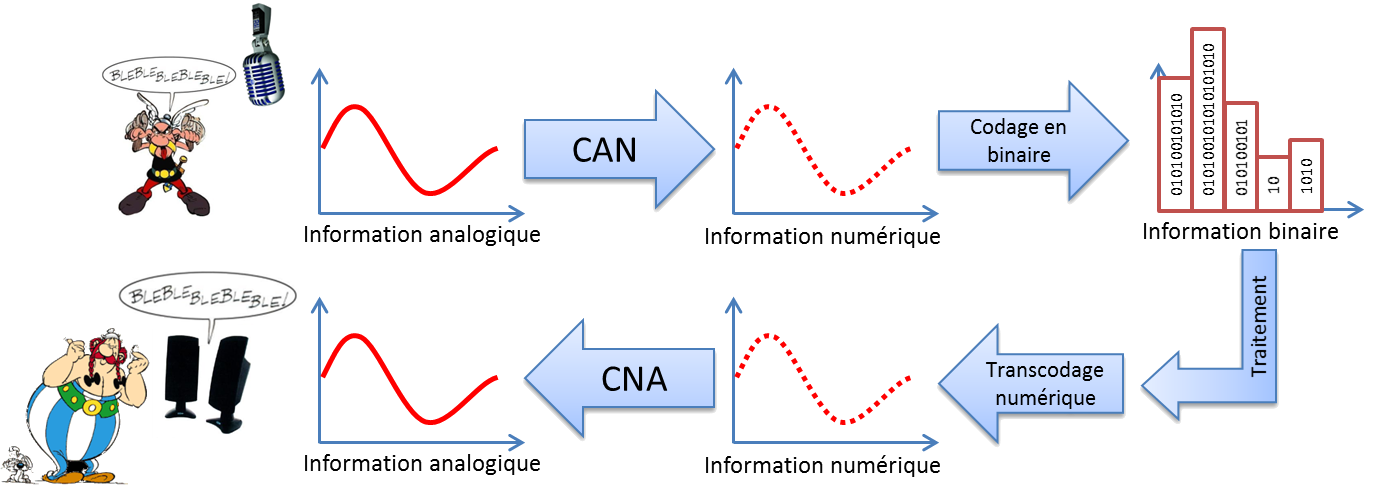
\includegraphics[width=.8\linewidth]{CAN_CNA}
\end{center}

\subsection{Echantillonnage et quantification}

\begin{defi}{Echantillonnage}
Échantillonner un signal consiste à prélever les valeurs de ce signal à intervalles définis. Si ces intervalles sont réguliers, on note $T_e$ la période d'échantillonnage (en seconde), c'est-à-dire la durée entre deux prélèvements. On note $f_e = \dfrac{1}{T_e}$ la fréquence d'écantillonnage (en Hertz), c'est-à-dire le nombre d'échantillons par seconde.

Si on note e(t) le signal continu, on notera $e_k = e(kT_e)$ la valeur de l'échantillon $e(t)$ à l'instant $kT_e$. 

\end{defi}

\begin{center}
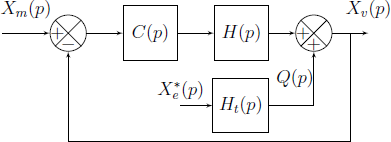
\includegraphics[width=.8\linewidth]{fig_03}
\end{center}

\begin{theorem}{\small{\textsf{\textbf{Théorème de Shannon}}}} ~\\
Soit un signal périodique décomposable en signaux périodiques dont la fréquence maximale présente est largement supérieure à celle minimale présente.
La représentation discrète d’un signal par des échantillons régulièrement espacés exige une fréquence d’échantillonnage supérieure au double de la fréquence maximale présente dans ce signal.
\end{theorem}

Dans le cas suivant, le signal est sinusoïdal de fréquence $\SI{1}{Hz}$. Avec un échantillonnage de \SI{1}{Hz} ou \SI{2}{Hz}, on prélève le signal lorsqu'il est nul. Il est donc opportun de prendre une fréquence d'échantillonnage plus grande afin de ne pas perdre d'information. 
\begin{center}
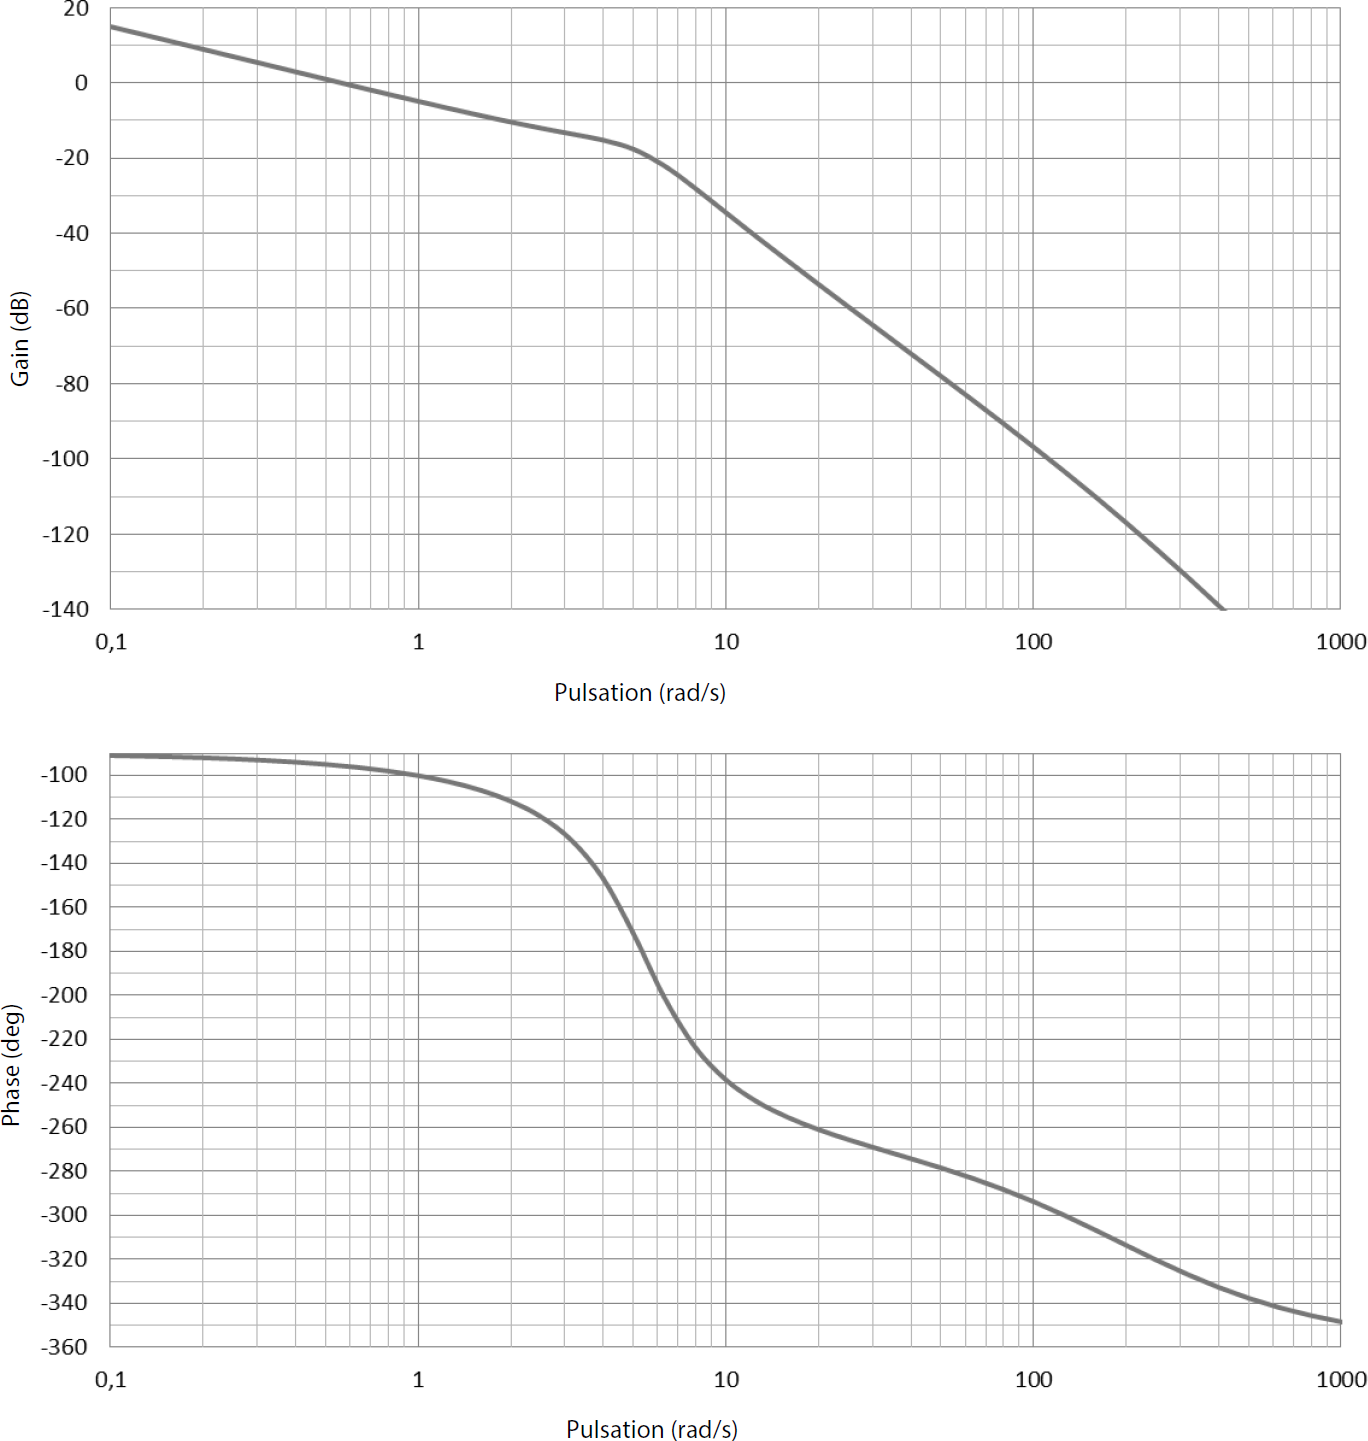
\includegraphics[width=.8\linewidth]{fig_04}
\end{center}




\begin{defi}{Quantification}
Quantifier in signal consiste à approcher un signal continu par les valeurs d'un ensemble discret. 

En général, le système étant échantilloné sur un système binaire sur $N$ bits, on peut donc approcher le signal par $2^N$ valeurs discrètes.
\end{defi}

La figure ci-dessous illustre un signal échantillonné à \SI{7}{Hz}. Il a ensuite été numérisé selon 4 niveaux de quantication. Plus le nombre de bits de codage est élevé, plus l'erreur entre signal numérisé et signal initial est faible.
 
\begin{center}
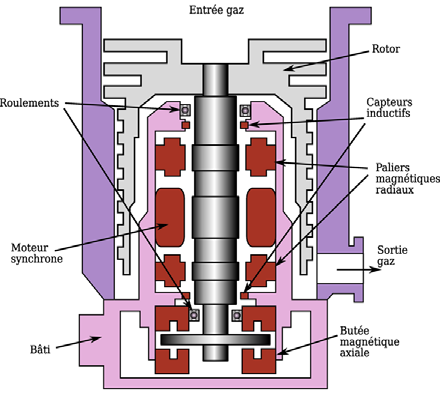
\includegraphics[width=.8\linewidth]{fig_05}
\end{center}


\begin{defi}{Erreur de quantification}
Soit un signal continu borné entre les valeurs $e_{\text{min}}$ et $e_{\text{max}}$ échantilloné sur $N$ bits. Le pas de quantification donne aussi l'erreur maximala de quantification. On a $q = \dfrac{e_{\text{max}}-e_{\text{min}}}{2^N}$.

\end{defi}


\subsection{Conversion analogique -- numérique}
La conversion analogique consiste, lors de l'acquisition d'un signal, à léchantillonner et le  numériser. 
\begin{defi}{Signal numérique}

Un signal numérique est un système échantillonné et quantifié. 

\end{defi}

\subsection{Conversion numérique -- analogique}
Le plus souvent, la conversion numérique -- analogique a pour but de synthétiser un signal de commande. Il va donc falloir passé d'un système quantifié échantillonné à un signal analogique. Le plus souvent, on utilise un bloqueur qui va maintenir la valeur $u_k$ de l'instant $k$ à l'instant $k+1$ (c'est à dire pendant la durée de la période d'échantillonnage $T_e$). 

Mathématiquement, on utilise un bloqueur d'ordre 0 dont la fonction de transfert $B_0(p)$ est $B_0(p)=\dfrac{1-e^{-T_e p}}{p}$.

\begin{center}
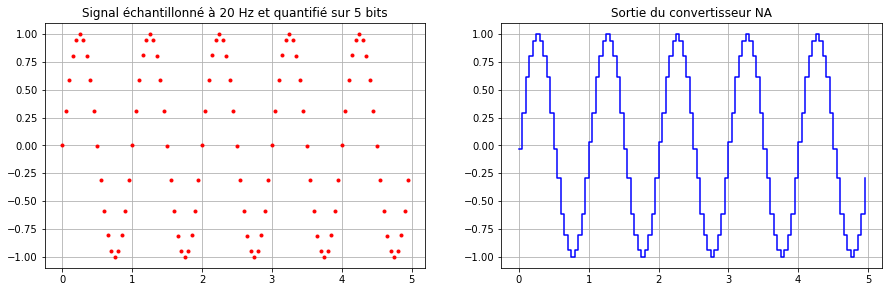
\includegraphics[width=.8\linewidth]{fig_06_CNA}
\end{center}

\section{Filtrage numérique}
Lors de l'acquisition de signaux, le signal numérique issu du convertsisseur numérique est (quasiment toujours) bruité. 
De ce fait, il est nécessaire de le filtrer pour supprimer ce bruit, sans pour autant déformer le signal utilie. 

\begin{defi}{Filtrage numérique}~\\
\begin{minipage}[c]{.7\linewidth}
Soit $e_k$ un signal discret. Soit $s_k$ un signal discret filtré. $k\in \mathbb{N}$ est le numéro de l'échantillon. On appelle filtrage numérique l'opération mathématique permettant de filtrer un signal, c'est-à-dire d'éliminer certaines composantes harmoniques. 
\end{minipage} \hfill
\begin{minipage}[c]{.25\linewidth}
\begin{center}
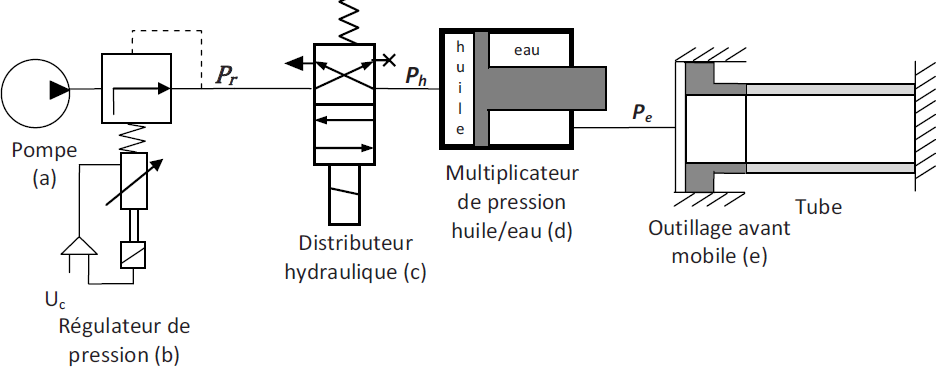
\includegraphics[width=\linewidth]{fig_01}
\end{center}
\end{minipage}
\end{defi}

\subsection{Filtrage numérique passe-bas}
\begin{defi}{Filtre passe-bas du premier ordre}~\\
On donne l'équation différentielle d'un filtre du premier ordre : $s(t)+\tau \deriv{s(t)}{} = e(t)$.  $T_e$ est la période d'échantillonnage du système. La pulsation de coupure à $-\SI{3}{dB}$ du filtre est donné par $\omega_c = \dfrac{1}{\tau}$.

On montre que $s_k = \dfrac{T_e}{T_e+\tau} e_k + \dfrac{\tau}{T_e+\tau} s_{k-1}$ avec $T_e$ période d'échantillonnage du système.  
\end{defi}

\begin{demo}
On a  $s(t)+\tau \deriv{s(t)}{} = e(t)$. En approximant $\deriv{s(t)}{}$ par $\dfrac{s(t) -s(t-T_e)}{T_e}$, puis en discrétisant l'équation différentielle, on a donc : 
 $s_k +\tau \dfrac{s_k - s_{k-1}}{T_e} = e_k$
 $\Leftrightarrow s_k \left(1+\dfrac{\tau}{T_e}\right) - s_{k-1}\dfrac{\tau}{T_e} = e_k$
 $\Leftrightarrow s_k \dfrac{T_e+\tau}{T_e}  = e_k + s_{k-1}\dfrac{\tau}{T_e}$
 $\Leftrightarrow s_k   = e_k \dfrac{T_e}{T_e+\tau}+ s_{k-1}\dfrac{\tau}{T_e}\dfrac{T_e}{T_e+\tau}$
 $\Leftrightarrow s_k   = e_k \dfrac{T_e}{T_e+\tau}+ s_{k-1}\dfrac{\tau}{T_e+\tau}$.
\end{demo}

\begin{minipage}[c]{.48\linewidth}
Caractéristiques du signal bruité :
\begin{itemize}
\item $s(t)=\sin(t) + 0,1\sin(2\pi \times 10 t)+ 0,05\sin(2\pi \times 100 t)$.
\end{itemize}
\end{minipage}
\begin{minipage}[c]{.48\linewidth}
\begin{center}
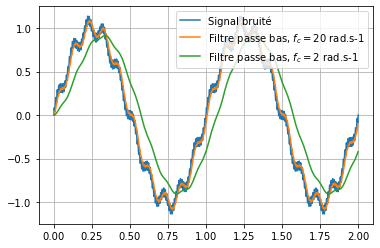
\includegraphics[width=\linewidth]{fig_07_filtrePB.png}
\end{center}
\end{minipage}


\subsection{Filtrage numérique à moyenne glissante} 


\begin{minipage}[c]{.48\linewidth}
Pour réaliser un filtrage à moyenne glissante, le signal filtré $f_k$ à l'instant $k$ est égale à le moyenne des $N$ précédentes valeurs du signal $s_k$. On a donc, $\forall k \geq N-1, f_k = \dfrac{1}{N}\sum\limits_{i=0}^{N-1} s_{k-i}$.

Pendant les $N-1$ premiers instants le signal filtré est donc à l'état nul. Ce filtre induit donc un retard temporel.

Caractéristiques du signal bruité :
\begin{itemize}
\item $s(t)=\sin(t) + 0,1\sin(2\pi \times 10 t)+ 0,05\sin(2\pi \times 100 t)$.
\end{itemize}
\end{minipage}
\begin{minipage}[c]{.48\linewidth}
\begin{center}
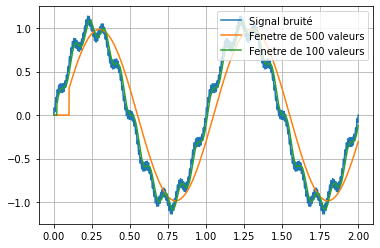
\includegraphics[width=\linewidth]{fig_08_moyenneg.png}
\end{center}
\end{minipage}

\section{Correcteurs numériques}
 
 Les systèmes asservis utilisés sont en réalité le plus souvent numérique. Ainsi, le calcul de l'écart et la correction sont 
 réalisés sous formes numériques par le microcontrôleur, la carte d'axe ou l'automate. 
 
 \begin{center}
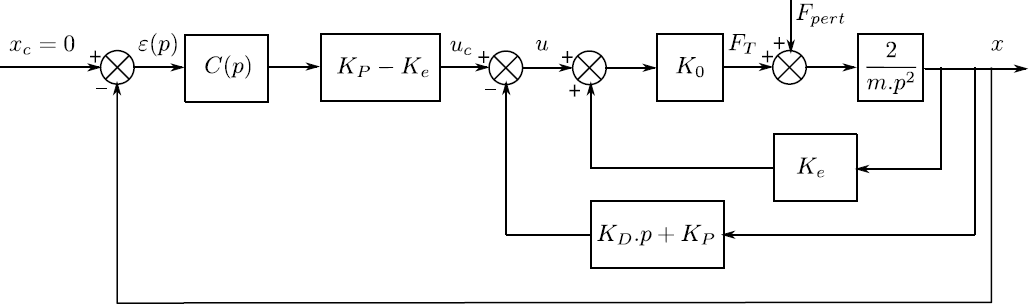
\includegraphics[width=\linewidth]{fig_02}
\end{center}

Ainsi le correcteur numérique va devoir synthétiser la commande numérique $u_k$ en fonction de l'écart $\varepsilon_k$. 


 
\subsection{Correcteur P}
\begin{defi}{Correcteur proportionnel}
Dans le domaine temporel, on a $u(t)=K_P \varepsilon(t)$. Cela est traduit par le relation de récurrence suivante : 
$u_k = K_p \varepsilon_k$.
\end{defi}
\subsection{Correcteur PI}
\begin{defi}{Correcteur proportionnel intégral}
Dans le domaine temporel, on a $u(t)=K_P  \left(\varepsilon(t)+\dfrac{1}{T_i}\int\limits_0^t \varepsilon(\tau) \dd \tau \right)$. Cela est traduit par le relation de récurrence suivante : 
$u_k = u_{k-1} +  K_p \left( \varepsilon_k \left( 1+\dfrac{T_e}{T_i}\right) - \varepsilon_{k-1} \right)$.
\end{defi}

\begin{demo}
Pour déterminer la relation de récurrence, il faut calculer $\int\limits_0^t \varepsilon(\tau) \dd \tau$. 
Pour cela, si on utilise la méthode des rectangles à droite, on a 
$\int\limits_0^t \varepsilon(\tau) \dd \tau \simeq \sum\limits_{j=1}^k \varepsilon_j T_e$; donc 
$u_k = K_p\left(\varepsilon_k + \dfrac{T_e}{T_i}\sum\limits_{j=1}^k \varepsilon_j \right)$.

Par ailleurs, à l'instant $k-1$, $u_{k-1} = K_p\left(\varepsilon_{k-1} + \dfrac{T_e}{T_i}\sum\limits_{j=1}^{k-1} \varepsilon_j \right)$


Cherchons une relation entre $u_{k-1}$ et $u_{k}$ : 
$u_k = K_p\left(\varepsilon_k + \dfrac{T_e}{T_i}\sum\limits_{j=1}^{k-1} \left(\varepsilon_j \right) + \dfrac{T_e}{T_i} \varepsilon_k \right)$

$= K_p\left(\varepsilon_k \left(1+\dfrac{T_e}{T_i}\right)+ \dfrac{T_e}{T_i}\sum\limits_{j=1}^{k-1} \left(\varepsilon_j \right) + \varepsilon_{k-1} - \varepsilon_{k-1}\right)$

$= K_p\left(\varepsilon_k \left(1+\dfrac{T_e}{T_i}\right) - \varepsilon_{k-1}\right)
+ K_p\left(\dfrac{T_e}{T_i}\sum\limits_{j=1}^{k-1} \left(\varepsilon_j \right) + \varepsilon_{k-1} \right) $
$= K_p\left(\varepsilon_k \left(1+\dfrac{T_e}{T_i}\right) - \varepsilon_{k-1}\right) + u_{k-1} $. \textit{CQFD.}
\end{demo}


\subsection{Correcteur PID}
\begin{defi}{Correcteur proportionnel intégral et dérivé}

Dans le domaine temporel, on a $u(t)=K_P  \left(\varepsilon(t)+\dfrac{1}{T_i}\int\limits_0^t \varepsilon(\tau) \dd \tau +T_d \dfrac{\dd \varepsilon(t)}{\dd t}\right)$. Cela est traduit par le relation de récurrence suivante : 
$u_k = u_{k-1} + K_p \left( \varepsilon_k \left( 1+\dfrac{T_e}{T_i}+\dfrac{T_d}{T_e}\right) - \varepsilon_{k-1} \left( 1+\dfrac{T_d}{T_e}\right)\right)$.

\end{defi}

\begin{demo}
On a déjà vu que pour un correcteur PI, $u_k = K_p\left(\varepsilon_k \left(1+\dfrac{T_e}{T_i}\right) - \varepsilon_{k-1}\right) + u_{k-1} $.

Par ailleurs, $T_d  \dfrac{\dd \varepsilon(t)}{\dd t} \simeq T_d  \dfrac{\varepsilon_k -\varepsilon_{k-1}}{T_e}$. 
On a donc 
 $u_k = K_p\left(\varepsilon_k \left(1+\dfrac{T_e}{T_i}\right) - \varepsilon_{k-1}\right) + u_{k-1}  + K_p  T_d  \dfrac{\varepsilon_k -\varepsilon_{k-1}}{T_e} $
 

$= K_p\left(\varepsilon_k \left(1+\dfrac{T_e}{T_i}\right) - \varepsilon_{k-1} +  T_d  \dfrac{\varepsilon_k -\varepsilon_{k-1}}{T_e}\right) + u_{k-1}   $

$= K_p\left(\varepsilon_k \left(1+\dfrac{T_e}{T_i}+\dfrac{T_d}{T_e}\right) - \varepsilon_{k-1}\left( 1+\dfrac{T_d}{T_e}\right) \right) + u_{k-1}   $

\end{demo}

%
%\section{Limite des correcteurs lors de la commande de systèmes}
%
%\begin{thebibliography}{2}
%%   \bibitem[1]{ref1} Frédéric Mazet, {\it Cours d'automatique de deuxième année, Lycée Dumont Durville, Toulon.}
%%   \bibitem[2]{ref2} Florestan Mathurin, {\it Correction des SLCI, Lycée Bellevue, Toulouse, \url{http://florestan.mathurin.free.fr/}.}
%%   \bibitem[3]{ref3} Damien Iceta, David Violeau, Alain Caignot, Xavier Pessoles, Vincent Boyer, François Golanski, {\it Sciences industrielles de l'ingénieur MP/MP* PSI/PSI* PT/PT*, Méthodes. Exercices. Problèmes. Sujets de concours. Vuibert Prépas.}
%\end{thebibliography}





